%%%%%%%% ICML 2023 EXAMPLE LATEX SUBMISSION FILE %%%%%%%%%%%%%%%%%

\documentclass{article}

% Recommended, but optional, packages for figures and better typesetting:
\usepackage{microtype}
\usepackage{graphicx}
\usepackage{subfigure}
\usepackage{booktabs} % for professional tables

\usepackage{tikz}
% Corporate Design of the University of Tübingen
% Primary Colors
\definecolor{TUred}{RGB}{165,30,55}
\definecolor{TUgold}{RGB}{180,160,105}
\definecolor{TUdark}{RGB}{50,65,75}
\definecolor{TUgray}{RGB}{175,179,183}

% Secondary Colors
\definecolor{TUdarkblue}{RGB}{65,90,140}
\definecolor{TUblue}{RGB}{0,105,170}
\definecolor{TUlightblue}{RGB}{80,170,200}
\definecolor{TUlightgreen}{RGB}{130,185,160}
\definecolor{TUgreen}{RGB}{125,165,75}
\definecolor{TUdarkgreen}{RGB}{50,110,30}
\definecolor{TUocre}{RGB}{200,80,60}
\definecolor{TUviolet}{RGB}{175,110,150}
\definecolor{TUmauve}{RGB}{180,160,150}
\definecolor{TUbeige}{RGB}{215,180,105}
\definecolor{TUorange}{RGB}{210,150,0}
\definecolor{TUbrown}{RGB}{145,105,70}

% hyperref makes hyperlinks in the resulting PDF.
% If your build breaks (sometimes temporarily if a hyperlink spans a page)
% please comment out the following usepackage line and replace
% \usepackage{icml2023} with \usepackage[nohyperref]{icml2023} above.
\usepackage{hyperref}


% Attempt to make hyperref and algorithmic work together better:
\newcommand{\theHalgorithm}{\arabic{algorithm}}

\usepackage[accepted]{icml2023}

% For theorems and such
\usepackage{amsmath}
\usepackage{amssymb}
\usepackage{mathtools}
\usepackage{amsthm}

% if you use cleveref..
\usepackage[capitalize,noabbrev]{cleveref}

%%%%%%%%%%%%%%%%%%%%%%%%%%%%%%%%
% THEOREMS
%%%%%%%%%%%%%%%%%%%%%%%%%%%%%%%%
\theoremstyle{plain}
\newtheorem{theorem}{Theorem}[section]
\newtheorem{proposition}[theorem]{Proposition}
\newtheorem{lemma}[theorem]{Lemma}
\newtheorem{corollary}[theorem]{Corollary}
\theoremstyle{definition}
\newtheorem{definition}[theorem]{Definition}
\newtheorem{assumption}[theorem]{Assumption}
\theoremstyle{remark}
\newtheorem{remark}[theorem]{Remark}

% Formular
\usepackage{array,tabularx}
\newenvironment{conditions*}
  {\par\vspace{\abovedisplayskip}\noindent
   \tabularx{\columnwidth}{>{$}l<{$} @{\ : } >{\raggedright\arraybackslash}X}}
  {\endtabularx\par\vspace{\belowdisplayskip}}

% Quelle
\newcommand*{\quelle}{
  \footnotesize Imagesource: Inverted image from\\
}

% Todonotes is useful during development; simply uncomment the next line
%    and comment out the line below the next line to turn off comments
%\usepackage[disable,textsize=tiny]{todonotes}
\usepackage[textsize=tiny]{todonotes}


% The \icmltitle you define below is probably too long as a header.
% Therefore, a short form for the running title is supplied here:
\icmltitlerunning{Project Report Template for Data Literacy 2023/24}

\begin{document}

\twocolumn[
\icmltitle{The Evolution of Complexity in Lego Sets}

% It is OKAY to include author information, even for blind
% submissions: the style file will automatically remove it for you
% unless you've provided the [accepted] option to the icml2023
% package.

% List of affiliations: The first argument should be a (short)
% identifier you will use later to specify author affiliations
% Academic affiliations should list Department, University, City, Region, Country
% Industry affiliations should list Company, City, Region, Country

% You can specify symbols, otherwise they are numbered in order.
% Ideally, you should not use this facility. Affiliations will be numbered
% in order of appearance and this is the preferred way.
\icmlsetsymbol{equal}{*}

\begin{icmlauthorlist}
\icmlauthor{Edward Beach}{equal,first}
\icmlauthor{Patricia Schlegel}{equal,second}
\end{icmlauthorlist}

% fill in your matrikelnummer, email address, degree, for each group member
\icmlaffiliation{first}{Matrikelnummer 5451904, edward.beach@student.uni-tuebingen.de, MSc Cognitive Science}
\icmlaffiliation{second}{Matrikelnummer 5480232, patricia.schlegel@student.uni-tuebingen.de, MSc Cognitive Science}

% You may provide any keywords that you
% find helpful for describing your paper; these are used to populate
% the "keywords" metadata in the PDF but will not be shown in the document
\icmlkeywords{Machine Learning, ICML}

\vskip 0.3in
]

% this must go after the closing bracket ] following \twocolumn[ ...

% This command actually creates the footnote in the first column
% listing the affiliations and the copyright notice.
% The command takes one argument, which is text to display at the start of the footnote.
% The \icmlEqualContribution command is standard text for equal contribution.
% Remove it (just {}) if you do not need this facility.

%\printAffiliationsAndNotice{}  % leave blank if no need to mention equal contribution
\printAffiliationsAndNotice{\icmlEqualContribution} % otherwise use the standard text.

\begin{abstract}

In our Data Literacy project, we aimed to determine if the complexity of Lego sets has been increasing since the beginning of Lego production. Using exponential and linear regression, as well as cluster analysis, our findings consistently indicated a noticeable upward trend in set complexity over the years.

\end{abstract}

\section{Introduction}\label{sec:intro}
As Lego enthusiasts and researchers, we wanted to work with a Lego dataset. After an exploratory analysis of the dataset we saw that different numbers such as mean number of total parts per set, mean number of different parts and unique parts, number of colors and minifigures increased over the years. We started to wonder, if we could say that the complexity of Lego sets in terms of production increased over the years. \\

Value ...

\\

In the following sections, we detail the methods and data used for our complexity analysis. This involves a comprehensive exploration of the Rebrickable dataset, encompassing details on Lego sets released between 1949 and 2024. We describe the formulation of the complexity metric, its normalization, and the subsequent linear and exponential regressions modeling for predicting mean complexity per year until 2030. Additionally, a k-means clustering analysis is detailed, outlining the optimal number of clusters based on the complexity metric.


\section{Data and Methods}\label{sec:methods}

For our project we used the \href{https://rebrickable.com/downloads/}{Rebrickable dataset} spanning Lego Sets from 1949 to 2024. The dataset contains details on 17.077 sets, 35.408 parts, 13.546 minifigures, 144 themes, 251 colors and 66 part categories, organized into several CSV files and classes (see Figure 1).

\begin{figure}[ht]
 \vskip 0.2in
 \begin{center}
 \centerline{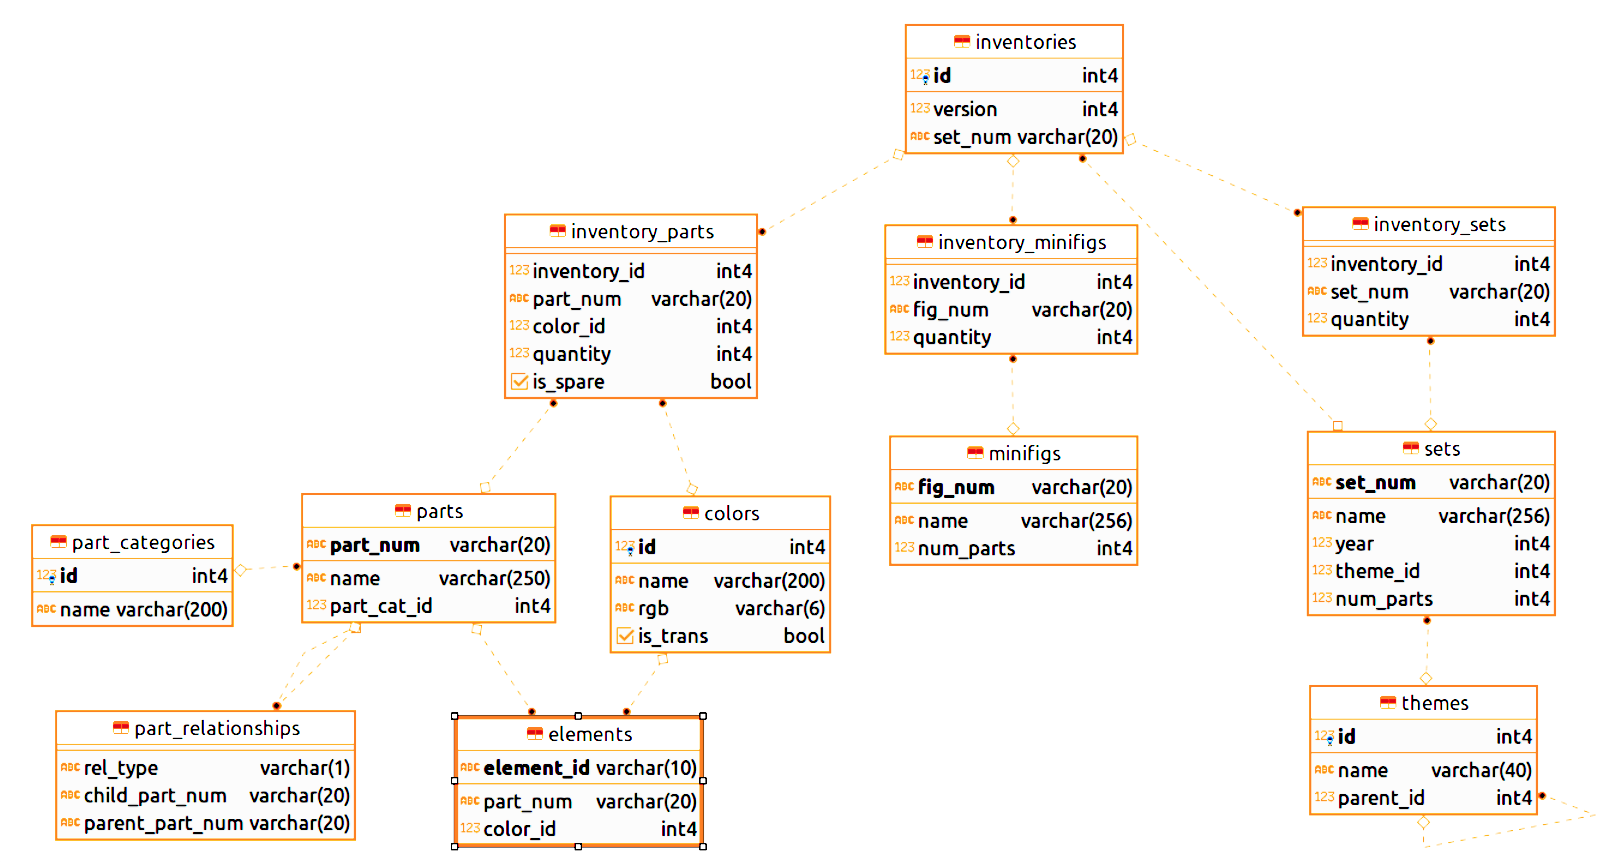
\includegraphics[width=\columnwidth]{inverted_database.png}}
 \quelle\url{https://rebrickable.com/downloads/}
\caption{Structure of the Rebrickable Dataset}
\label{icml-historical}
 \end{center}
 \vskip 0.1in
\end{figure}



Everything was implemented in python and can be found in a \href{https://github.com/eddiebeach99/Data_Literacy/tree/development}{git repository}. In our analysis used the "sklearn" libary for regression and clustering. \\
The initial data processing involved merging classes into two comprehensive datasets. The first integration combined part categories with parts, yielding an extensive list of detailed part information. Subsequently, categories, parts, inventory parts, and colors were integrated to form a dataset detailing parts within inventories, including color specifications. For the second dataset, the minifigs class were merged with inventory minifigs to extract specific information about minifigures within inventories. The dataset was refined by filtering themes for main themes and establishing connections between sets and themes.\\
In the subsequent merging phase, the sets with themes dataset was combined with datasets containing information about parts and minifigures, resulting in two distinct datasets – one focused on parts in different sets and there characteristics and the other on minifigures in different sets. To maintain relevance, the datasets were filtered to include only data up to the year 2023, ensuring the incorporation of completed years.\\
The final step involved creating a consolidated dataset by grouping data using the set number. The grouped dataset included pertinent details for each set such as release year, theme, total number of part and number of different parts, minifigure quantities, color diversity, category variety, counts of unique parts (quantity of one in the set), and the proportion of unique to not unique parts within each set.\\
After data preparation, we started to explore the data to discern trends in Lego set features over the years. The following deeper exploration involved analyzing the mean proportion of unique parts to non-unique parts per set per year. Additionally, the ten most used themes between 2000 and 2023 were identified using different criteria (number of sets, number of parts, most different parts) and furthermore determined the most used ten colors in those themes. Predictions for these metrics and the number of released sets and mean part count per set until 2030 were made using linear regression. These analyses can be found in the \href{https://github.com/eddiebeach99/Data_Literacy/blob/main/Analysis/exploratory_analysis.ipynb}{exploratory analysis file on github}. \\
After that we got an intuition about the dataset and moved to the main analysis. We introduce a complexity metric for each set. Because we want to examine the complexity in terms of production complexity we used factors such as the total number of parts and number of different parts, the different part categories, the number of unique parts, the number different colors, and number of minifigures. This complexity metric aimed to quantify the intricacy of production, considering the varied materials/colors, number of parts that have to be produced and different manufacturing processes required. We therefore propose the following formula for the production complexity:

\[
Comp = Parts + Diff + Cat + Uniq + Col + Figs
\]
where
\begin{conditions*}
 Comp & Complexity\\
 Parts  &  Total number of parts\\
 Diff  &  Number of different parts \\
 Cat & Number of different categories of the parts\\
 Uniq  & Number of unique parts \\
 Col & Number of different colors\\
 Figs & Number of minifigures\\
\end{conditions*}

The complexity metric was then normalized to a range between 0 and 1, enhancing interpretability. Normalization was achieved by applying the formula:\\

\[Complexity = \frac{Comp - MinComp}{MaxComp - MinComp}\]\\
where
\begin{conditions*}
 Complexity & Normalized complexity\\
 Comp & Complexity\\
 MinComp  &  Minimal complexity across all sets\\
 MaxComp  &  Maximal complexity across all sets \\
\end{conditions*}

Subsequently, a linear and exponential regression was employed to model the mean complexity per year, providing predictions until 2030. We compared the Sum of Squared Residuals (SSR) and Coefficient of Determination ($R^2$) to find the regression that better fits the data.\\
Additionally, a k-means clustering analysis, guided by the elbow method, was conducted to determine the optimal number of clusters based on the complexity metric.



% This is the template for a figure from the original ICML submission pack. In lecture 10 we will discuss plotting in detail.
% Refer to this lecture on how to include figures in this text.
% 
% \begin{figure}[ht]
% \vskip 0.2in
% \begin{center}
% \centerline{\includegraphics[width=\columnwidth]{icml_numpapers}}
% \caption{Historical locations and number of accepted papers for International
% Machine Learning Conferences (ICML 1993 -- ICML 2008) and International
% Workshops on Machine Learning (ML 1988 -- ML 1992). At the time this figure was
% produced, the number of accepted papers for ICML 2008 was unknown and instead
% estimated.}
% \label{icml-historical}
% \end{center}
% \vskip -0.2in
% \end{figure}

\section{Results}\label{sec:results}
We started with an exploratory phase were we plotted different features of Lego sets. For each year we plotted the number of released sets, mean part count per set, mean different parts per set, mean minifigures per set, themes per year, mean part categories per set, mean colors per set, the number of different colors, and mean unique parts per set (see Figure 2).

\begin{figure}[ht]
 \vskip 0.2in
 \begin{center}
 \centerline{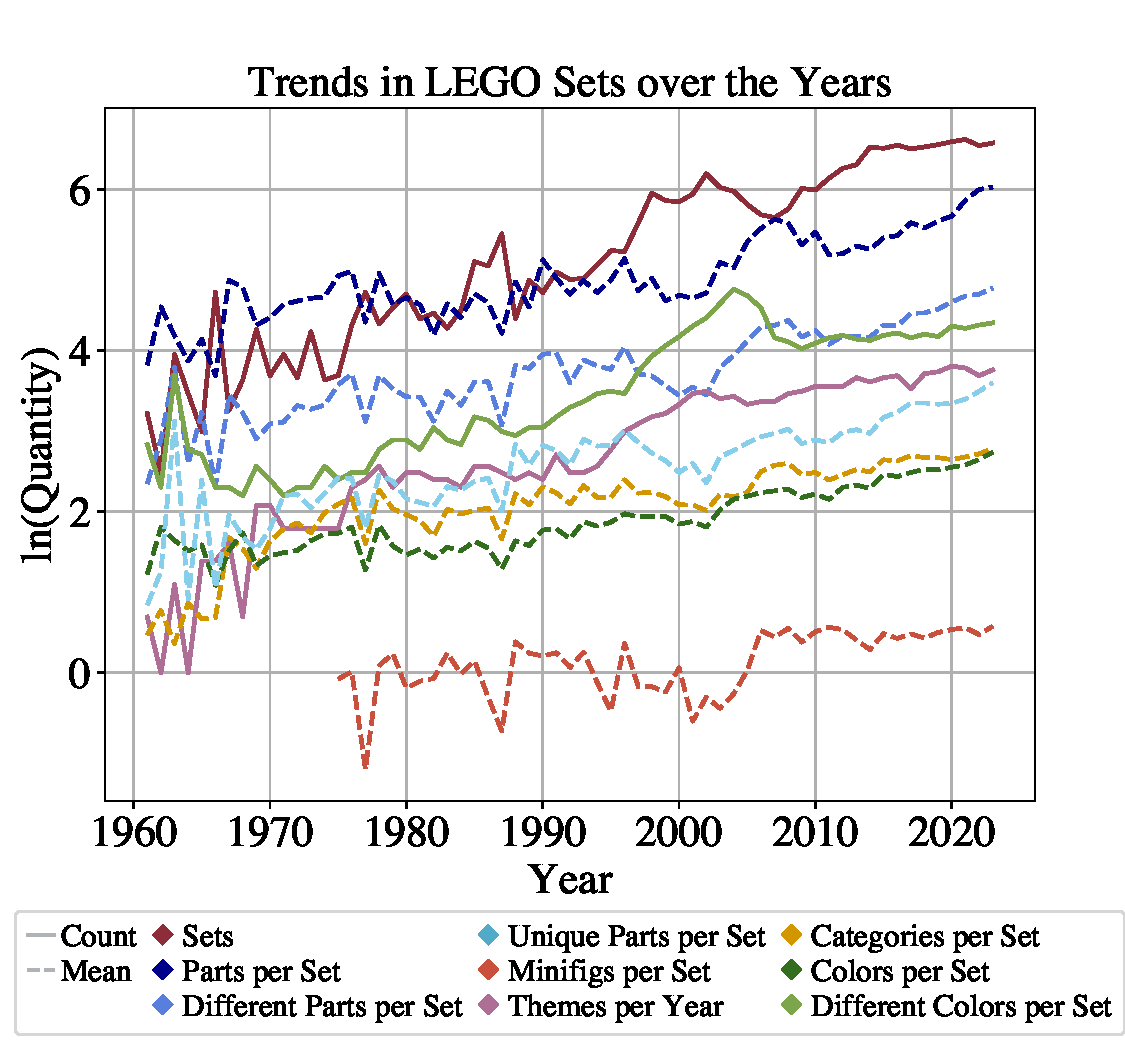
\includegraphics[width=\columnwidth]{Images/Exploration.pdf}}
\caption{Trends of different features of Lego sets over the years}
\label{icml-historical}
 \end{center}
 \vskip -0.2in
\end{figure}

Afterwards we focused our analysis on the complexity of the production of different Lego sets. We performed a linear regression ($SSR = 0.0039$, $R^2= 0.5742$) and exponential regression ($SSR = 0.0035$, $R^2= 0.6132$) for the average complexity per set per year with a prediction until 2030 (see Figure 3). Further visualisation can be found on \href{https://github.com/eddiebeach99/Data_Literacy/blob/main/Analysis/complexity_regression.ipynb}{github}.

\begin{figure}[ht]
 \vskip 0.2in
 \begin{center}
 \centerline{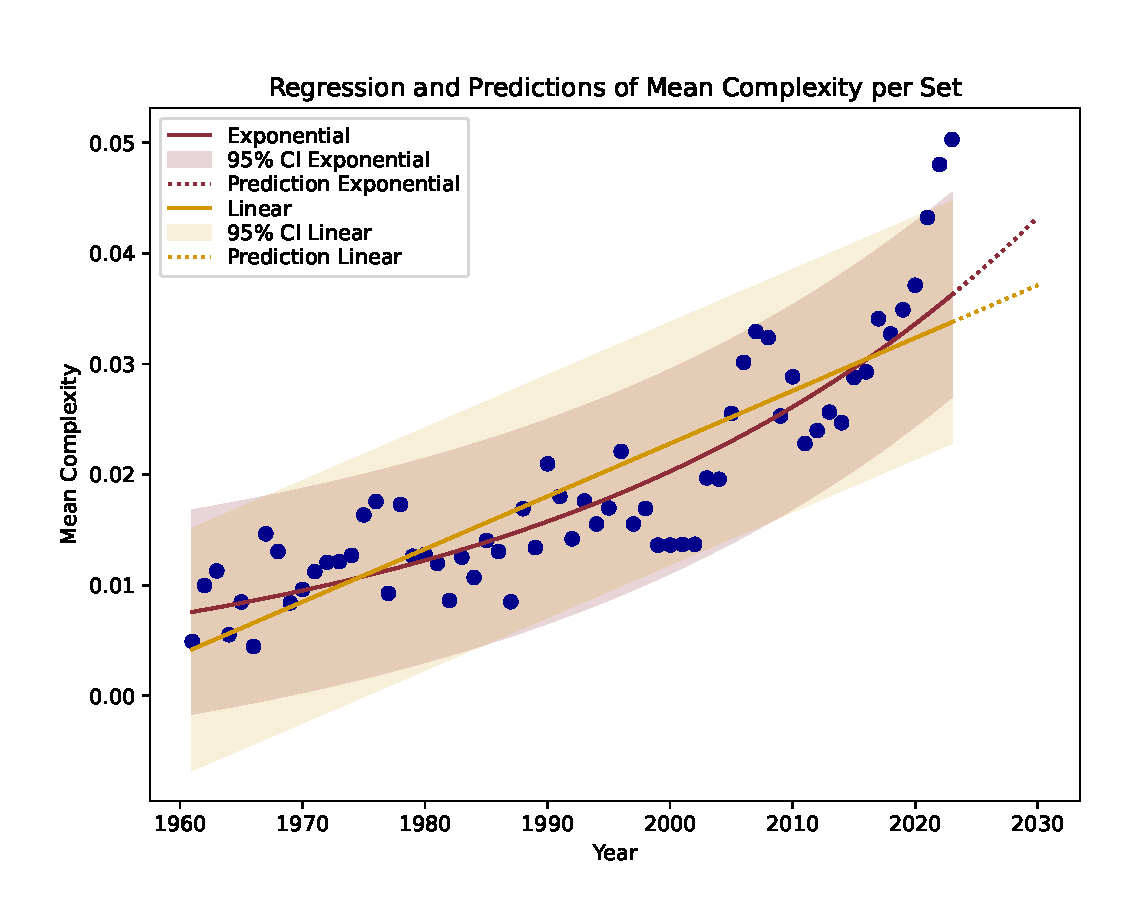
\includegraphics[width=\columnwidth]{Images/Regressions.pdf}}
\caption{Exponential and linear regression of the mean complexity for a Lego set per year with predictions until 2030}
\label{icml-historical}
 \end{center}
 \vskip -0.2in
\end{figure}

We then performed a k-means clustering, that aimed to group the data based on complexity with the elbow method, which set the optimal number of clusters to three. Afterwards we compared the average complexity scores in the different clusters (Cluster 0: $0.0599$, Cluster 1: $0.0092$, Cluster 2: $0.2685$), set the complexity level of the clusters from low to high (Cluster 0: Medium, Cluster 1: Low, Cluster 2: High) and visualized the distribution of sets across different clusters (see Figure 4). Further visualisation can be found on \href{https://github.com/eddiebeach99/Data_Literacy/blob/main/Analysis/clustering.ipynb}{github}.

\begin{figure}[ht]
 \vskip 0.2in
 \begin{center}
 \centerline{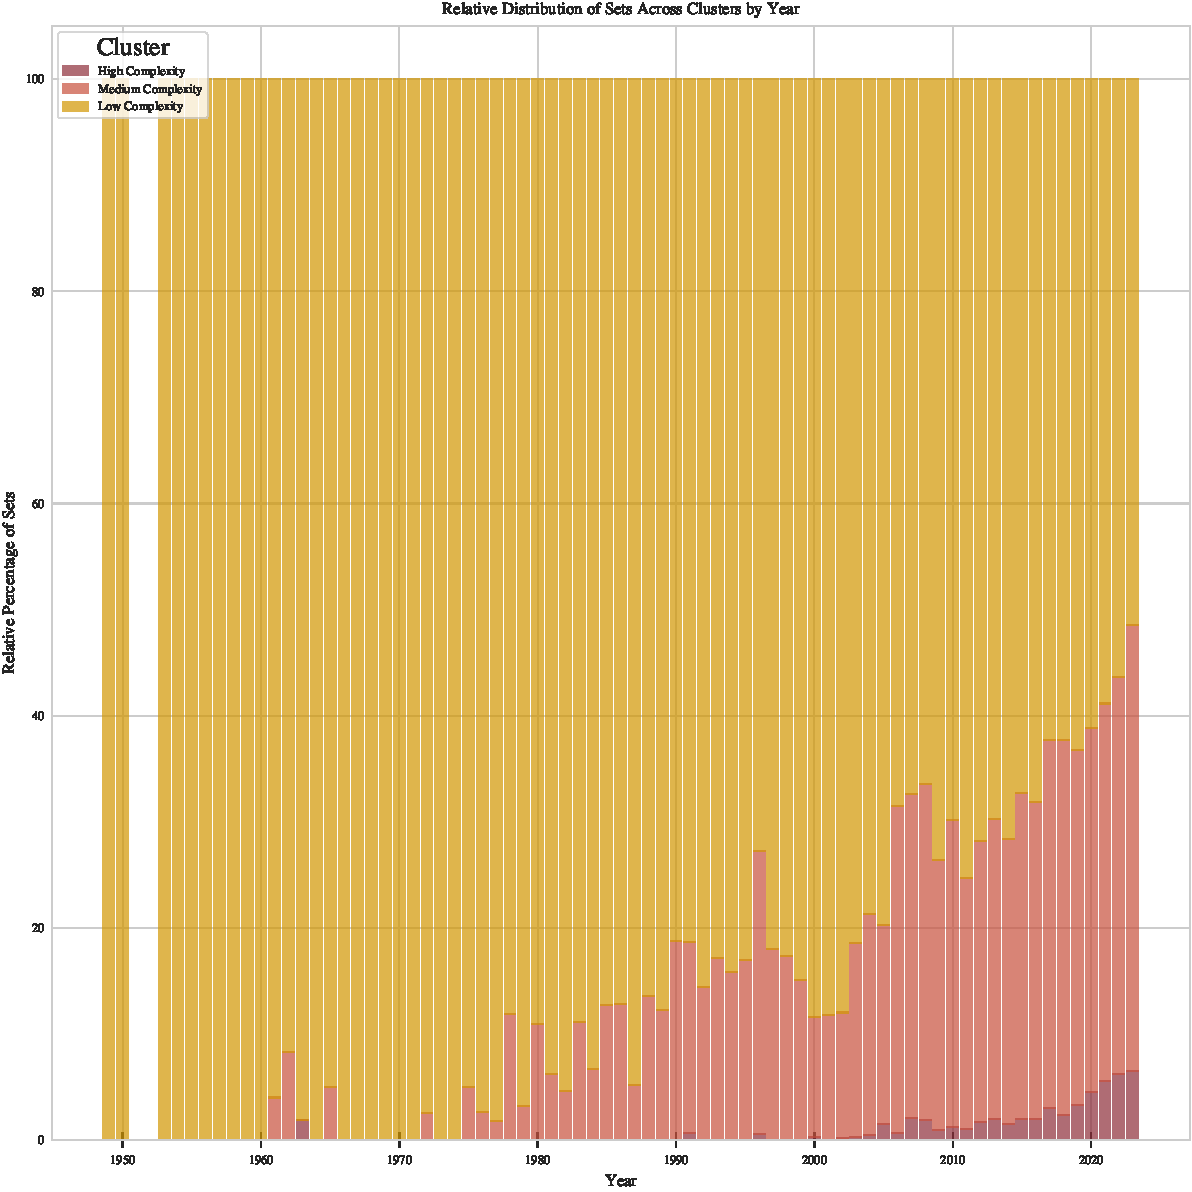
\includegraphics[width=\columnwidth]{Images/Clusters.pdf}}
\caption{Proportion of sets in the different clusters}
\label{icml-historical}
 \end{center}
 \vskip -0.2in
\end{figure}

\section{Discussion \& Conclusion}\label{sec:conclusion}

After data preparation, we started to explore the data to discern trends in Lego set features over the years. For each year we plotted the number of released sets, mean part count per set, mean different parts per set, mean minifigures per set, themes per year, mean part categories per set, mean colors per set, the number of different colors, and mean unique parts per set (see Figure 2). We can see that all the numbers are increasing over the years, which led us to suspect that the complexity Lego sets, in terms of production, could be increasing as well. \\
To test this hypothesis, we started to introduce a complexity measure in terms of production and calculated it for each set. We then calculated a linear and exponential regression for the mean complexity for a set. We can see for both regressions that the mean complexity is increasing and that the prediction of complexity is as well. We can also see that the exponential regression provides a better fit to the data, evidenced by a lower SSR and a higher $R^2$ value. \\
In the Cluster analysis of the proportion of sets in the different complexity levels, we can see similar findings. The complexity started really low but increased over the years. More and more sets started to be in the clusters with a medium and high complexity, while the number of sets with low complexity are decreasing. \\

A limitation is that the number of lego sets is increasing as well?

\section*{Contribution Statement}

Patricia Schlegel prepared data, calculated the complexity for each Lego set and made first exploratory analyses, which included the two regressions of the complexity. Edward Beach performed the k-means clustering and revised the plots for the report. All authors jointly wrote the text of the report.

\section*{Notes} 

Your entire report has a \textbf{hard page limit of 4 pages} excluding references. (I.e. any pages beyond page 4 must only contain references). Appendices are \emph{not} possible. But you can put additional material, like interactive visualizations or videos, on a githunb repo (use \href{https://github.com/pnkraemer/tueplots}{links} in your pdf to refer to them). Each report has to contain \textbf{at least three plots or visualizations}, and \textbf{cite at least two references}. More details about how to prepare the report, inclucing how to produce plots, cite correctly, and how to ideally structure your github repo, will be discussed in the lecture, where a rubric for the evaluation will also be provided.


\bibliography{bibliography}
\bibliographystyle{icml2023}

\end{document}


% This document was modified from the file originally made available by
% Pat Langley and Andrea Danyluk for ICML-2K. This version was created
% by Iain Murray in 2018, and modified by Alexandre Bouchard in
% 2019 and 2021 and by Csaba Szepesvari, Gang Niu and Sivan Sabato in 2022.
% Modified again in 2023 by Sivan Sabato and Jonathan Scarlett.
% Previous contributors include Dan Roy, Lise Getoor and Tobias
% Scheffer, which was slightly modified from the 2010 version by
% Thorsten Joachims & Johannes Fuernkranz, slightly modified from the
% 2009 version by Kiri Wagstaff and Sam Roweis's 2008 version, which is
% slightly modified from Prasad Tadepalli's 2007 version which is a
% lightly changed version of the previous year's version by Andrew
% Moore, which was in turn edited from those of Kristian Kersting and
% Codrina Lauth. Alex Smola contributed to the algorithmic style files.
